% Lecture Template for ME3001-001-Tristan Hill - Spring 2017
% 
% Mechanical Engineering Analysis with MATLAB
%
% Systems of Linear Equations - Lecture 5 - Eigenvalues


% Document settings
\documentclass[11pt]{article}
\usepackage[margin=1in]{geometry}
\usepackage[pdftex]{graphicx}
\usepackage{multirow}
\usepackage{setspace}
\usepackage{hyperref}
\usepackage{color,soul}
\usepackage{fancyvrb}
\usepackage{framed}
\usepackage{wasysym}
\usepackage{multicol}

\pagestyle{plain}
\setlength\parindent{0pt}
\hypersetup{
    bookmarks=true,         % show bookmarks bar?
    unicode=false,          % non-Latin characters in Acrobat’s bookmarks
    pdftoolbar=true,        % show Acrobat’s toolbar?
    pdfmenubar=true,        % show Acrobat’s menu?
    pdffitwindow=false,     % window fit to page when opened
    pdfstartview={FitH},    % fits the width of the page to the window
    pdftitle={My title},    % title
    pdfauthor={Author},     % author
    pdfsubject={Subject},   % subject of the document
    pdfcreator={Creator},   % creator of the document
    pdfproducer={Producer}, % producer of the document
    pdfkeywords={keyword1} {key2} {key3}, % list of keywords
    pdfnewwindow=true,      % links in new window
    colorlinks=true,       % false: boxed links; true: colored links
    linkcolor=red,          % color of internal links (change box color with linkbordercolor)
    citecolor=green,        % color of links to bibliography
    filecolor=magenta,      % color of file links
    urlcolor=blue           % color of external links
}

% assignment number 

\definecolor{mygreen}{rgb}{0, .39, 0}

%\definecolor{dred}{#8B0000}
% [153,50,204] - dark orchid
\definecolor{mypurple}{rgb}{0.6,0.1961,0.8}
%[139,69,19] - saddle brown
\definecolor{mybrown}{rgb}{0.5451,0.2706,0.0745}

\definecolor{mygray}{rgb}{.6, .6, .6}

\setulcolor{red} 
\setstcolor{green} 
\sethlcolor{mygray} 

\newcommand{\VA}{\vspace{2mm}}
\newcommand{\VB}{\vspace{5mm}} 
\newcommand{\VC}{\vspace{30mm}} 
 
\newcommand{\R}{\color{red}}
\newcommand{\B}{\color{blue}}
\newcommand{\K}{\color{black}}
\newcommand{\G}{\color{mygreen}}
\newcommand{\PR}{\color{mypurple}}

\newcommand{\NUM}{1} 
\newcommand{\VSpaceSize}{2mm} 
\newcommand{\HSpaceSize}{2mm} 

\begin{document}

\textbf{ \LARGE ME 3001 Lecture - Eigenvalues and Eigenvectors} \\\\
\textbf{ \LARGE The Magic Numbers!} \\

\begin{itemize}

	\item  \textbf{\LARGE What is an Eigenvector? Eigenvalue?}\\\\
\Large{
	In linear algebra, an eigenvector or characteristic vector of a linear transformation is a non-zero vector whose direction does not change when that linear transformation is applied to it. More formally, if $T$ is a linear transformation from a vector space $V$ over a field $F$ into itself and $v$ is a vector in $V$ that is not the zero vector, then $v$ is an eigenvector of $T$ if $T(v)$ is a scalar multiple of $v$. This condition can be written as the equation\\

\scalebox{1.5}{$T({\bf v})=\lambda{\bf v}$}\\

where $\lambda$ is a scalar in the field $F$, known as the eigenvalue, characteristic value, or characteristic root associated with the eigenvector $v$.

If the vector space $V$ is finite-dimensional, then the linear transformation $T$ can be represented as a square matrix $A$, and the vector $v$ by a column vector, rendering the above mapping as a matrix multiplication on the left hand side and a scaling of the column vector on the right hand side in the equation.\\


\scalebox{1.5}{$[A]{\bf v}=\lambda{\bf v}$}\\

\item  \textbf{\LARGE That makes sense right?}\\\\

\newpage
\item  \textbf{\LARGE The Standard Form of the Eigenvalue problem.}\\

 
%\begin{itemize}
		The Equations \\\\ 
		  \scalebox{1.25}{$(a_{11}-\lambda) x_1 + a_{12} x_{2} + ... + a_{1n} x_n = 0 $} \vspace{2mm}\\
		  \scalebox{1.25}{$a_{21} x_1 + (a_{22}-\lambda)  x_{2} + ... + a_{2n} x_n = 0 $} \\
		  \scalebox{1.25}{$\hspace{20mm}.$}\\
		  \scalebox{1.25}{$\hspace{20mm}.$}\\
		  \scalebox{1.25}{$a_{n1} x_1 + a_{n2} x_{2} + ... + (a_{nn}-\lambda) x_n = 0 $} \\	
		  
		 The Matrix Form 	\\
		 	\scalebox{1.25}{\parbox{.5\linewidth}{
			\[ \left( \begin{array}{cccc}
			(a_{11}-\lambda)  & a_{12} & ...& a_{1n} \\
			a_{21} & (a_{22}-\lambda)  & ...& a_{2n} \\
			&.&&\\
			&.&&\\
			a_{n1} & a_{n2} & ...& (a_{nn}-\lambda) \end{array} \right) \times \left[ \begin{array}{c}
			x_1 \\
			x_2 \\
			.\\
			.\\
			x_n \end{array} \right] = \left[ \begin{array}{c}
			0\\
			0 \\
			.\\
			.\\
			0 \end{array} \right]\] 
			}}
			 
		 	\scalebox{1.25}{\parbox{.5\linewidth}{
			\[ \left(\left[ \begin{array}{cccc}
			a_{11}  & a_{12} & ...& a_{1n} \\
			a_{21} & a_{22}  & ...& a_{2n} \\
			&.&&\\
			&.&&\\
			a_{n1} & a_{n2} & ...& a_{nn} \end{array} \right]-\lambda\left[ \begin{array}{cccc}
			1  & 0 & ...& 0 \\
			0 & 1  & ...& 0 \\
			0 & 0  & 1 & 0 \\
			&.&&\\
			0 & 0 & ...& 1 \end{array} \right]\right) \times \left[ \begin{array}{c}
			x_1 \\
			x_2 \\
			.\\
			.\\
			x_n \end{array} \right] = \left[ \begin{array}{c}
			0\\
			0 \\
			.\\
			.\\
			0 \end{array} \right]\] 
			}}

		 	\scalebox{1.25}{\parbox{.5\linewidth}{
			\[ \left( \begin{array}{cccc}
			a_{11}  & a_{12} & ...& a_{1n} \\
			a_{21} & a_{22}  & ...& a_{2n} \\
			&.&&\\
			&.&&\\
			a_{n1} & a_{n2} & ...& a_{nn} \end{array} \right) \times \left[ \begin{array}{c}
			x_1 \\
			x_2 \\
			.\\
			.\\
			x_n \end{array} \right] = \lambda\left[ \begin{array}{c}
			x_1 \\
			x_2 \\
			.\\
			.\\
			x_n \end{array} \right]\] 
			}}

\newpage
\item  \textbf{\LARGE Let us look at the second matrix form more closely}\\\\

\scalebox{1.5}{$([A]-\lambda[I])\{x\}=\{0\}$} \\

First we need to realize that this matrix system is {\it Homogenous}. This follows a different rule regarding the existence of a solution.\\\\
 A {\it Homogeneous} system has a non-trivial solution if and only if the determinant of the coefficent matrix is zero.\\\\

\scalebox{1.5}{$|[A]|=0$}\\\\

Therefore, a solution to \scalebox{1.25}{$([A]-\lambda[I])\{x\}=\{0\}$} exists if...\\\\
\scalebox{1.5}{$|[A]-\lambda[I]|=0$} \\\\

This leads to a long $n^{th}$ order polynomial in terms of $\lambda$. This will have $n$ roots which may be real or complex.
\newpage
\item  \textbf{\LARGE 3x3 Example - A Vector in 3D} \\\\

For this we need the Determinant of a 3x3.\\

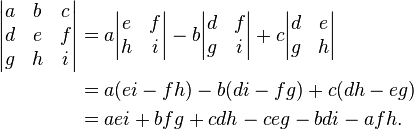
\includegraphics[scale=1]{lecture7_fig1.png} \\

And for the Eigenvalue problem the determinant becomes...\\\\

\scalebox{1}{$(a-\lambda)(e-\lambda)(i-\lambda)+bfg+cdh-c(e-\lambda)g-bd(i-\lambda)-(a-\lambda)fh$}\\\\

Lets add some numbers.\\\\


\newpage
\item  \textbf{\LARGE This concept can be visualized graphically!}\\\\


%\end{itemize}

}
\end{itemize}


	

\end{document}



